\problemname{Excursion to Porvoo}

It is a lovely summer day, and Alice wants to do a day trip. She lives in
Tampere, and wants to travel to Porvoo to enjoy the Old Town and the surrounding
nature. Alice does not only love travelling, but also planning.

She has created a map of the most beautiful paths to Porvoo. On her trip she
needs to visit $n$ cities in order, where Tampere is the first city and Porvoo
is the last city. The cities are connected by roads, with each road connecting
two consecutive cities, and there is always at least one road between each pair
of consecutive cities.

When driving from one city to the next, Alice needs to choose which road to take.
Some of these roads have a tarmac surface, while others are just gravel roads
and some roads have bridges which will not support vehicles that are too heavy.
For each road it is known how long it takes to traverse it and what is the
maximal weight of vehicles that can safely drive on it.

\begin{figure}[!h]
  \centering
  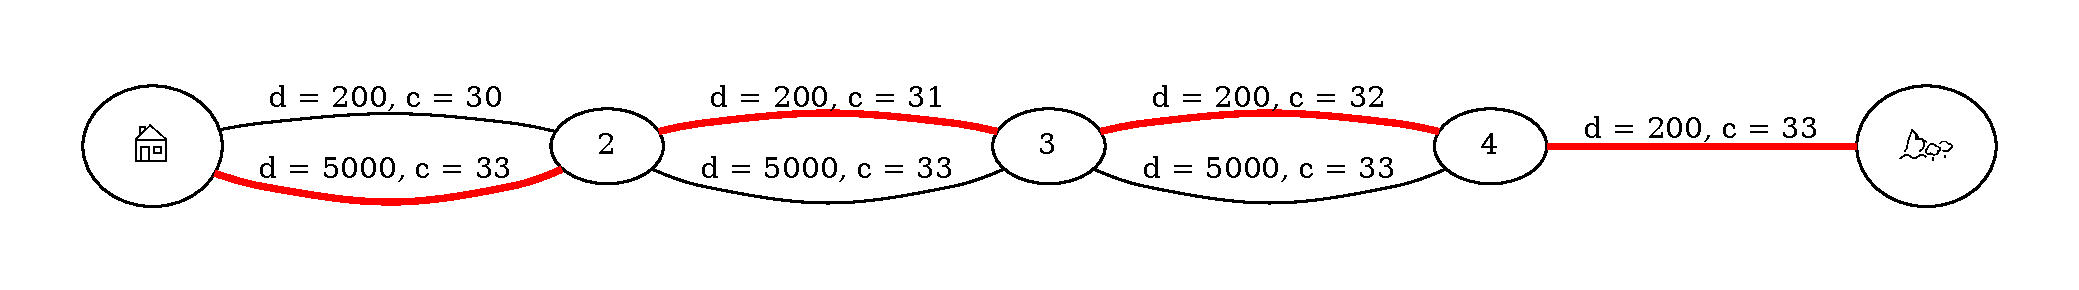
\includegraphics[width=1\textwidth]{sample2}
	\caption{Illustration of the second sample input. The red path from Tampere
	to Porvoo is the optimal choice for a car of weight $31$.}
\end{figure}

Alice collects many different cars of different weights,
but she is not sure yet which car she will use for the day trip.
As she wants to enjoy as much time in Porvoo as possible, she wants you to help
her find the minimal travel time for each car.

\section*{Input}
The input consists of:
\begin{itemize}
	\item Two integers $n$ and $m$ $(2 \leq n \leq 10^5, n - 1 \leq m \leq 10^5)$,
		the number of cities and the number of connections, respectively.
    The cities are numbered from $1$ to $n$, Tampere is city $1$, and Porvoo is city $n$.
	\item $m$ lines, each containing three integers $i$, $d$ and $c$ $(1 \leq i < n, 1
		\leq d \leq 10^4, 1 \leq c \leq 10^6)$, which each describe a connection
    between city $i$ and city $i + 1$ which takes $d$ minutes to traverse and
    can can be used by vehicles of weight $c$ kilograms or less.
	\item One integer $q$ $(1 \leq q \leq 10^5)$, the number of cars that Alice
		has collected.
	\item $q$ lines, where the $i$th line contains one integer $w_i$ $(1 \leq
		w_i \leq 10^6)$, the weight of the $i$th car in kilograms.
\end{itemize}

There is at least one connection from city $i$ to city $i+1$ for each $i$ ($1 \le i < n$).

\section*{Output}
Output $q$ lines, where the $i$th line describes the shortest time in minutes Alice
needs to drive to get from Tampere to Porvoo with the $i$th car.
If there is no feasible path for the $i$th car, output \texttt{impossible}.
